\chapter{Formalisms for language systems and language strategies}
\label{s:formalisms}

Modelling a language strategy encompasses defining semantic and
syntactic templates and applying realised templates that make up a
language system. Moreover, the language strategy needs to define
adoption, alignment and invention operators. This imposes hard
requirements on the formalisms that are needed to model a language
strategy.

Standard first-order formalisms in logic that are commonly used in
artificial language evolution research, such as predicate logic, are
insufficient to represent the semantic templates of some of the
strategies outlined in the previous chapter. For example, the meaning
of a realisation of the graded membership strategy, such as \textit{very
red}, cannot be expressed using any first-order logical formalism in
a satisfactory way as the the adverb \textit{very} modifies the meaning of
the adjective \textit{red}.

The syntactic templates require a grammar formalism, as the word order
seems to have an impact on the resulting focal colour that is
intended.  This is for example the case in the compounding strategy in
Russian, where \textit{zel\"eno-\v z\"eltyj} (`green-yellow') is different
from\textit{\v z\"elto-zel\"enyj} (`yellow-green'). This difference implies
that the lexical approach in which the lexicon captures a direct
association between terms and colour category is no longer sufficient.

In this book, I have chosen to use \emph{Incremental Recruitment
  Language} (IRL) to represent semantic templates and \emph{Fluid
  Construction Grammar} (FCG) to represent syntactic templates. Both
formalisms have been especially designed to support experiments in
artificial language evolution \citep{loetzsch09understanding}.

This chapter provides a short introduction to both systems that
introduces the design principles behind these formalisms and that
should enable the reader to understand the models of language
strategies that will be presented in future chapters. Readers can
choose to skip this chapter and return to it when needed.

\section{Embodied cognitive semantics using IRL}
\label{s:irl}
\is{Incremental Recruitment Language|see{IRL}}
\is{IRL}

\subsection{Theoretical foundations}

Although research on the emergence of communication systems with
similar features as human natural language has shown important
progress, the complexity of the meanings considered so far remains
limited. Experiments either use simple categories
\citep{steels05coordinating, belpaeme05explaining}, conjunctive
combinations of categories \citep{wellens08flexible} or
predicate-argument expressions \citep{batali02negotiation,
  smith03iterated, debeule08emergence}. Natural languages are clearly
capable of expressing second order semantics
\citep{dowty1981introduction}. For example, the adverb \textit{very} in
\textit{very big} modifies the meaning of the adjective, it is not just a
simple conjunction of the predicates \textit{very} and \textit{big}. Moreover the
same predicate (e.g. \textit{big}) can often be used in different ways, for
example to further restrict the set of possible referents of a noun
(as in \textit{the big ball}), to state a property of an object (as in
\textit{the ball is big}), to reify the predicate itself and make a
statement about it (as in \textit{big says something about size}), to
compare the elements of a set (as in \textit{this ball is bigger than the
others}), etc. The specific usage of a predicate in a particular
utterance is clearly conveyed by the grammar, so any theory on the
origins and evolution of grammar must address second order semantics.

The semantics of the utterances in this book are not represented in
a standard logic, but in an alternative framework, Incremental
Recruitment Language or IRL \citep{steels00emergence,
  steels05planning, vandenbroeck07constraintbased,
  vandenbroeck08constraintbased}. In this framework the meaning of a
sentence is a \emph{semantic constraint network} that the speaker
wants the hearer to evaluate in order to achieve the communicative
goal selected by the speaker. This approach resonates with earlier
work in AI on procedural semantics \citep{winograd72understanding}.

The IRL framework has been especially designed for experiments on
artificial language evolution and therefore supports key features that
have been proven successful in this field of research. It is
\emph{omni-directional}: not only can it be used for both
conceptualisation and interpretation but also to complete partial
semantic constraint networks. This feature does not only enable both
speaker and hearer to use the same formalism, but it has also proven
to be crucial when writing adoption, alignment and invention
operators. The speaker can use it to diagnose potential problems in
communication by interpreting its own utterance to detect potential
ambiguities \citep{steels03reentrance}. The hearer can try to
reproduce a partially understood meaning together with the
communicative goal, revealed by the speaker in a failed interaction,
to infer which parts it misinterpreted or did not know yet. On a
technical level, this strongly suggests a constraint-propagation
language \citep{marriott98programming}.

Another key feature of IRL is its \emph{open-endedness} towards the
cognitive operations it can represent. Previous research has deployed
a wide range of such operations including discrimination trees
\citep{steels96perceptually}, event feature detectors
\citep{siskind01grounding}, nearest neighbour classification
\citep{belpaeme05explaining} and radial basis function networks
\citep{steels05coordinating}.  IRL aims to be an overarching formalism
which can support any cognitive operation for which a tractable
implementation on a computer exists. It can be used for rich semantics
in which any of these operations can be combined and also for
experiments in which the choice of the cognitive operation is not
predetermined by the experimenter.

Finally, IRL is designed to support world models which are
\emph{grounded} in the sensory-motor system of the agent. These world
models are non-symbolic and are based on the operation of their
sensori-motor apparatus. Often \citep[e.g.][]{batali02negotiation,
  smith03iterated, wellens08flexible} it is assumed that there is a
simple straightforward mapping of the non-symbolic world model onto a
categorial situation model, which is a representation of the world in
the form of facts in some variant of predicate calculus. But as
different languages conceptualise the world in different ways, this
mapping function is clearly nontrivial.

\subsection{Semantic constraint network}
\label{s:semantic-constraint-network}
\is{semantic constraint network}
\is{semantic network|see{semantic constraint network}}

The meaning of an utterance will be viewed as a \textsc{semantic
  constraint network}, or \textsc{semantic network} for short. The basic
nodes of these networks are \textsc{primitive
  constraints}\is{primitive constraint} which reflect cognitive
operations and which are provided by the experimenter.  Each
constraint has a number of arguments which can be bound to a certain
variable. Variables are denoted using a question mark prefix. If a
variable appears as an argument to more than one constraint, it means
the value for this variable is constrained by more than one
constraint. Some variables can be bound to a certain \textsc{semantic
  entity}\is{semantic entity} by means of a bind
statement. Semantic entities are marked by square brackets.

An example network for an utterance like \textit{the block} is shown in
Figure \ref{f:context-and-network} to identify the block within a
hypothetical context. The {\sc Equal-to-Context} primitive (primitives
will always be printed in small capitals) binds all entities in the
context to $?s1$. The {\sc Filter-Set-Proto\-type} primitive takes
this entity-set as input, computes all entities that are similar to
the prototype of a block (provided by the bind statement through $?p1$)
and binds the resulting set to $?s2$. Finally, the {\sc
  Select-Element}, of which the selector is specified as [unique],
checks whether this set contains only one element and binds this
element to $?t$.

\begin{figure}
\centering
\subfigure[]{
  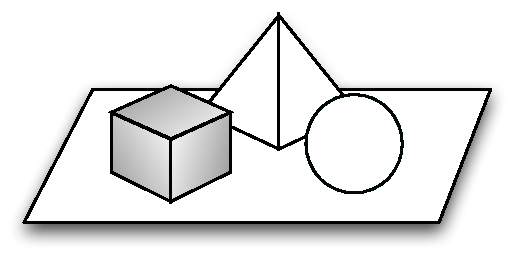
\includegraphics[width=0.45\textwidth]{./frameworks/figures/context.pdf}
  \label{f:context}
}
\subfigure[]{
  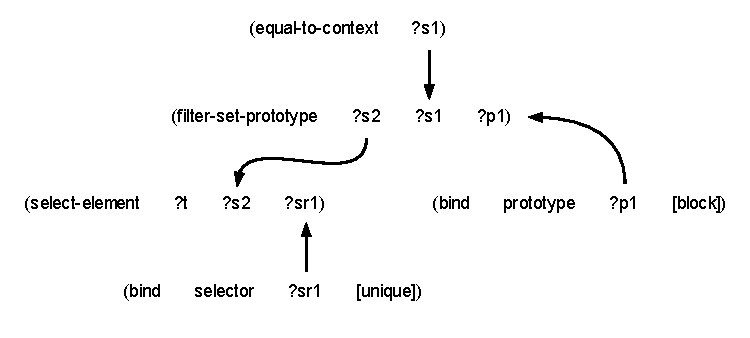
\includegraphics[width=\textwidth]{./frameworks/figures/network.pdf}
  \label{f:network}
}
\caption[Example semantic constraint network for \textit{the block}]{\subref{f:context} a hypothetical context \subref{f:network}
  an example of a semantic constraint network for \textit{the block} to
  identify the topic within (a) (marked in grey for clarity)}
\label{f:context-and-network}
\end{figure}

The more complex the world (for example by adding a second block), the
more complex the semantic constraint network will need to be in order
to achieve this goal (for example extending the previous one with
another filter operation based on size). An example of such a context
and such a network is shown in Figure
\ref{f:more-complex-context-and-network}. This network could represent
the meaning of an utterance like \textit{the big block}. The entity-set of
all blocks in $?s2$ is now further filtered to contain only big blocks
using the {\sc Filter-Set-Category} primitive, which binds the
resulting set to $?s3$ which is passed on to the {\sc Select-Element}
primitive. Note that the previous network in Figure \ref{f:network}
would fail in this context as the {\sc Select-Element} primitive with
a [unique] selector constrains the number of blocks in the context to
be one at most.

\begin{figure}[htbp]
\centering
\subfigure[]{
    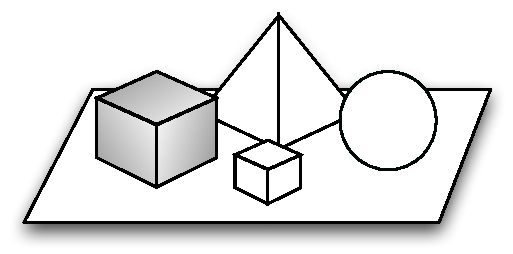
\includegraphics[width=.45\textwidth]{./frameworks/figures/more-complex-context.pdf}
  \label{f:more-complex-context}
}
\subfigure[]{
    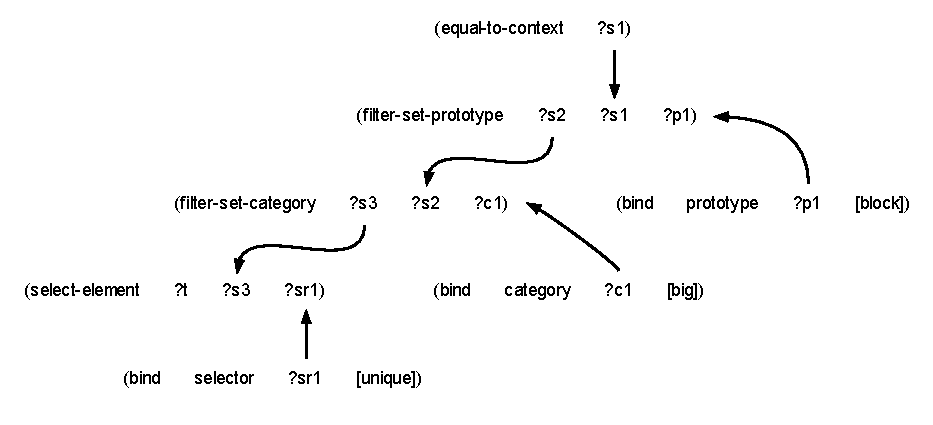
\includegraphics[width=\textwidth]{./frameworks/figures/more-complex-network.pdf}
  \label{f:more-complex-network}
}
\caption[Example semantic constraint network for \textit{the big
block}]{\subref{f:more-complex-context} a more complex hypothetical
  world \subref{f:more-complex-network} a more complex semantic
  constraint network to identify \textit{the big block} (marked in grey for
  clarity)}
\label{f:more-complex-context-and-network}
\end{figure}

\subsection{Evaluation}
\is{semantic constraint network!evaluation}

The evaluation of a semantic constraint network involves cycling
through the primitives of the network until each primitive has been
successfully revised. The revision of a primitive has three possible
outcomes: (1) validation with possible bindings for one or more of its
arguments (2) rejection or (3) suspension. Whenever a primitive
returns more than one possible solution, the evaluation tree which
keeps tracks of possible bindings for each variable in the network,
splits. This especially occurs during conceptualisation when the
semantic entities of the primitive constraints are still
unknown. Whenever a primitive rejects a particular set of bindings,
that particular branch in the evaluation tree can not be explored any
further. Whenever a primitive is not specified for a certain pattern
of bound or open arguments, it is suspended and revised at a later
moment.

During conceptualisation, the topic is typically known but the
semantic entities of the cognitive operators (like for example which
prototype or which category to use) are not. During interpretation,
the opposite is true: the semantic entities of the cognitive operators
have been passed on in the utterance, but the topic has not. A typical
network during interpretation is shown in Figure
\ref{f:more-complex-network}. The same network during
conceptualisation is shown in Figure
\ref{f:network-conceptualisation}.

The evaluation process of this network is shown in Figure
\ref{f:evaluation-process}. The context consists of four objects: a
big block (b-bk), a small block (s-bk), a ball (bl) and a pyramid (pd)
and the goal is to identify the big block in this context, so we have
a binding for $?t$. The only primitive that can be revised is {\sc
  Equal-to-Context} which can bind $?s1$ to the context: \{b-bk, s-bk,
bl, pd\}. The next primitive that can be revised is {\sc
  Filter-Set-Prototype} and let us suppose it knows the prototypes for
block and ball. This will cause a split in the evaluation tree: one in
which $?p1$ is bound to [block] and $?s2$ is bound to \{b-bk, s-bk\}
(node 2) and another branch in which $?p1$ is bound to [ball] and
$?s2$ is bound to \{bl\} (node 3). The next primitive that can be
revised is {\sc Filter-Set-Category}. Let us suppose this primitive is
only defined when its second argument contains at least two
entities. This will lead to a rejection of the branch of node 3 and to
a further split of the branch of node 2: one in which $?c1$ is bound
to [small] and $?s3$ is bound to \{s-bk\} (node 4) and another branch
in which $?c1$ is bound to [big] and $?s4$ is bound to \{b-bk\} (node
5). The final primitive that needs to be revised is {\sc
  Select-Element}, which checks whether $?s4$ contains only one entity
that is equal to the big block. This leads to a rejection of the
branch of node 4 but also to a successful evaluation of the branch of
node 5 in which $?sr1$ is bound to [unique].

\begin{figure}[htbp]
\centering
\subfigure[]{
    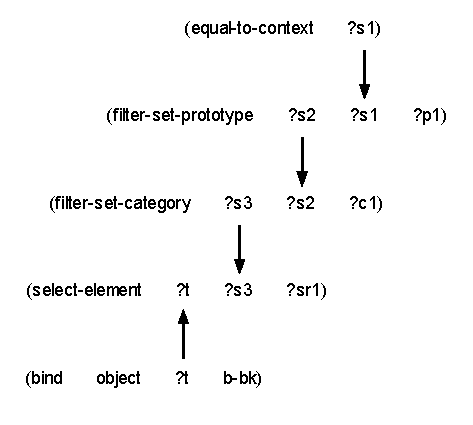
\includegraphics[width=.60\textwidth]{./frameworks/figures/network-conceptualisation.pdf}
  \label{f:network-conceptualisation}
}
\subfigure[]{
    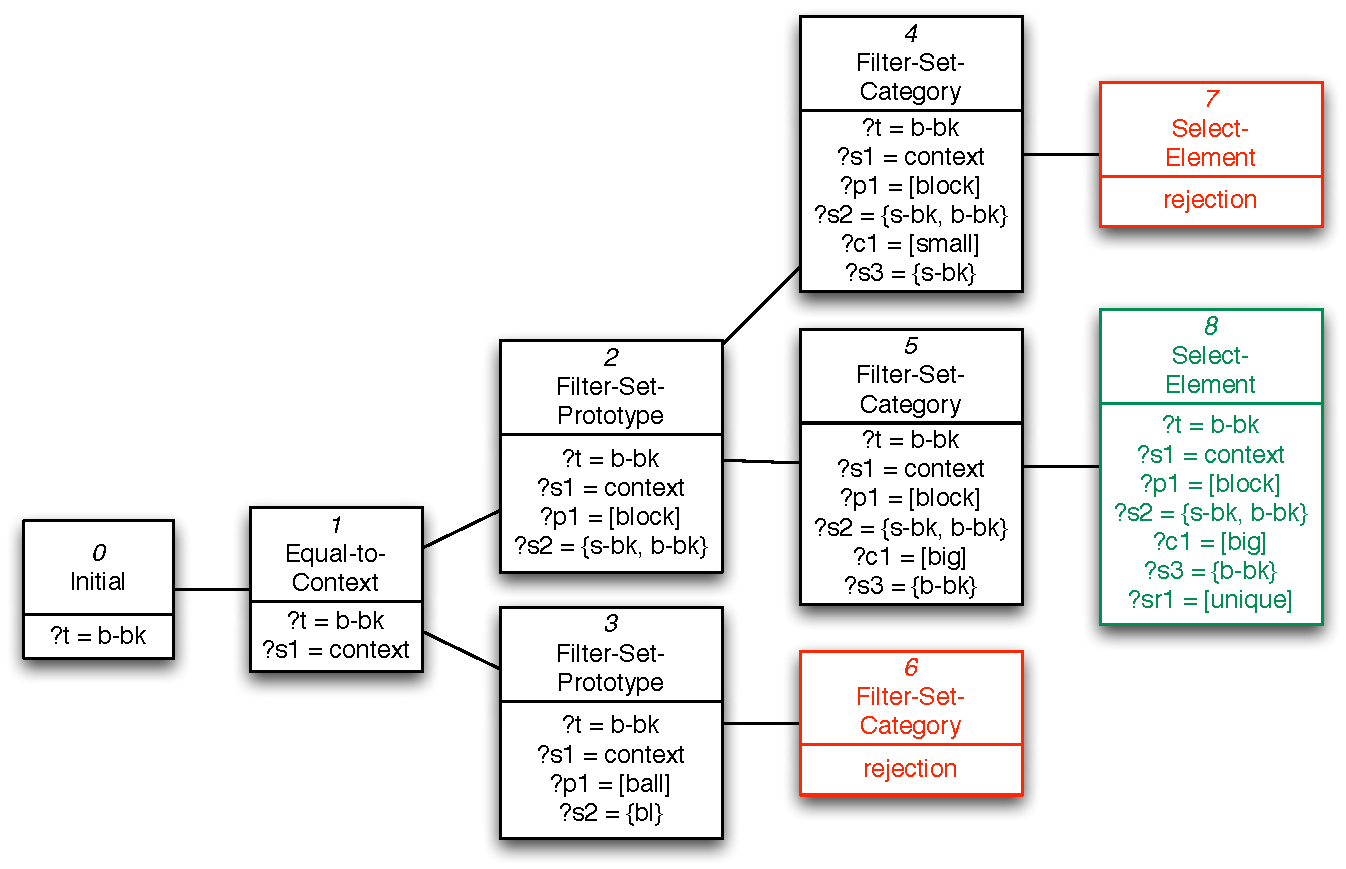
\includegraphics[width=.8\textwidth]{./frameworks/figures/evaluation.pdf}
  \label{f:evaluation-process}
}
\caption[Evaluation process of an example constraint
network]{\subref{f:evaluation-process} The evaluation process of an
  example network \subref{f:network-conceptualisation} during
  conceptualisation in a context consisting of four objects: a big
  block (b-bk), a small block (s-bk), a ball (bl) and a pyramid
  (pd). The communicative goal is to identify the big block.}
\label{f:evaluation}
\end{figure}

During acquisition of new semantic entities, the hearer will have been
able to reconstruct the intended semantic constraint network for a
large part. This network will be extended by the communicative goal
that is revealed by the speaker and will be revised in order to
acquire the semantic entity that fulfills the need in the current
network.

An example of such a network is shown in Figure
\ref{f:network-learning}, which could have been parsed after hearing a
sentence like \textit{the wabado ball}. Due to the omni-directional\-ity of
IRL, the first two arguments of the {\sc Filter-Set-Category}
primitive, $?s3$ and $?s2$ can be completely determined, which allows
IRL to come up with either a category that is already known or with an
entirely new category that would perform the correct filtering.

\begin{figure}[htbp]
  \begin{center}
    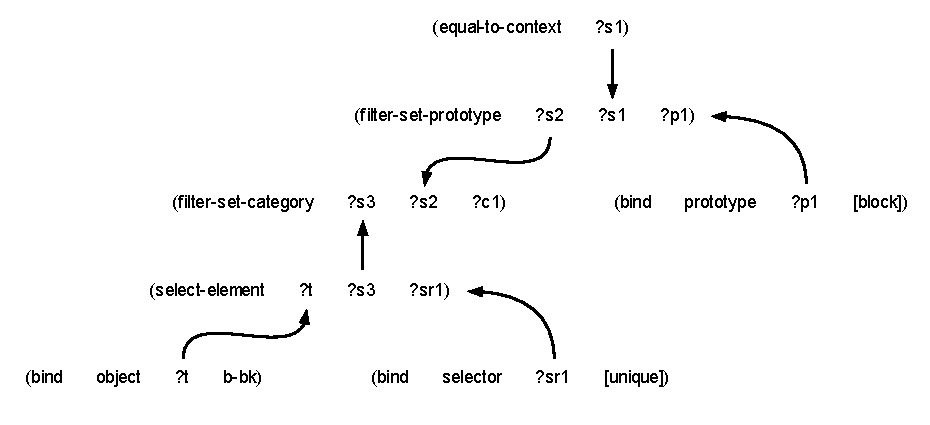
\includegraphics[width=\textwidth]{./frameworks/figures/network-learning.pdf}
    \caption[Example constraint network during learning]{A partial
      network that could be reconstructed by combining information
      from parsing \textit{the wabado ball} and the communicative goal
      revealed by the speaker. Due to the omni-directionality of IRL,
      the first two arguments of the {\sc Filter-Set-Category}
      primitive are sufficient to allow IRL to deduce a valid category
      for $?c1$.}
    \label{f:network-learning}
  \end{center}
\end{figure}

\subsection{Conceptualisation}
\label{s:irl-conceptualisation}
\is{conceptualisation}
\is{semantic constraint network!generation}

Conceptualisation can now be viewed as a search process in which a
semantic constraint network that is suitable to achieve the
communicative goal it selected \citep{steels05planning} needs be
constructed. Agents start with a library of primitive
constraints. These primitives are combined using heuristics to
construct networks that become more and more complex. In general,
these heuristics exploit the typical structure of the arguments of a
primitive and the type information of these arguments. The typical
structure is that the first argument is the target variable which can
be computed based on the values of the other arguments. Type
information is used to ensure that arguments that are linked are of
compatible type. More elaborate heuristics, which for example avoid
duplicate primitive constraints in one network, are also available.

An example of such a search process to identify a single object is
shown in Figure \ref{f:conceptualisation} which starts from a library
of four primitive constraints: {\sc Equal-to-Context}, {\sc
  Filter-Set-Prototype}, {\sc Filter-Set-Category} and {\sc
  Select-Element}. The search process starts from a variable bound to
the topic. This variable is considered to be an open variable for
which a primitive with a compatible target argument needs to be
found. Only one primitive in the library fulfils this requirement:
{\sc Select-Element}. This primitive again introduces an open variable
for its second argument which is of type entity-set. In the next
expansion step of the search tree, three primitives are considered:
{\sc Equal-to-Context}, {\sc Filter-Set-Prototype} and {\sc
  Filter-Set-Category} (nodes 2--4). Node 2 already contains a complete
network and can be evaluated. If the context contains only one object
this network succeeds and the conceptualisation process terminates. If
this is not the case, nodes 3 and 4 will be further expanded as they
again have an open variable of type entity-set. Both nodes can be
expanded with the three primitive constraints that have a compatible
target argument (nodes 5--10). If the topic can be identified using a
single {\sc Filter-Set-Prototype} (node 5) or {\sc
  Filter-Set-Category} (node 8), conceptualisation has been
completed. If not, the search process continues.

\begin{figure}
  \begin{center}
    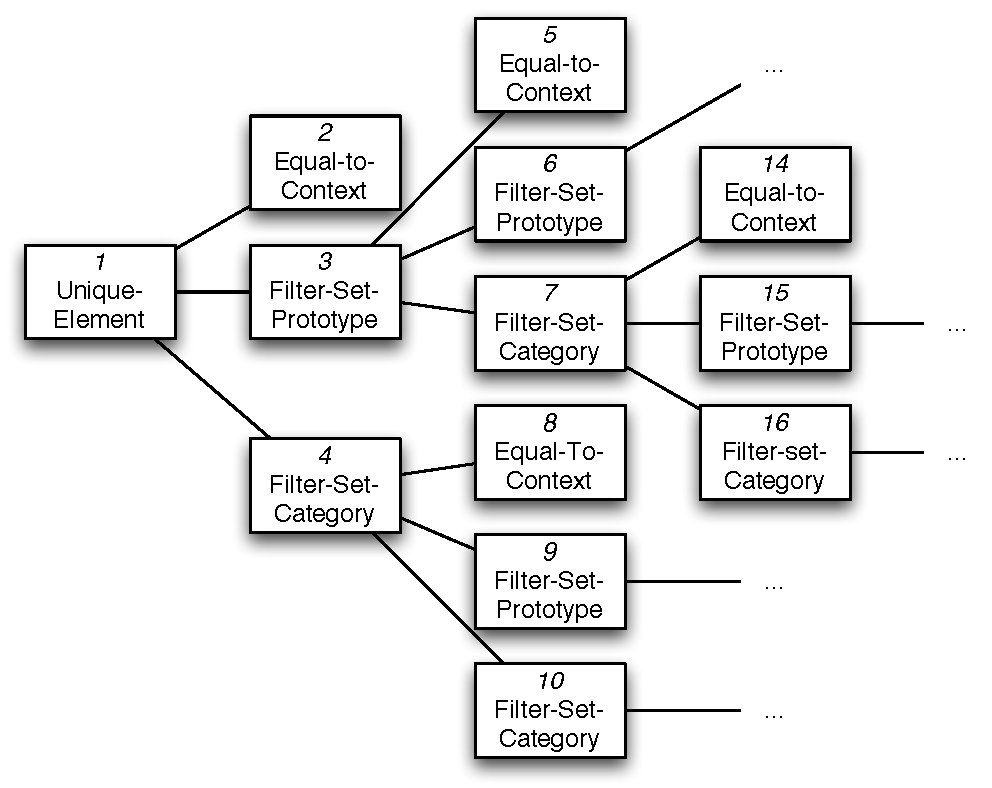
\includegraphics[width=.75\textwidth]{./frameworks/figures/conceptualisation.pdf}
    \caption[Example of the conceptualisation process]{Example search
      tree during conceptualisation, starting from a library of four
      primitives: {\sc Equal-to-Context}, {\sc Filter-Set-Prototype},
      {\sc Filter-Set-Category} and {\sc Select-Element}. The number
      in each node of this tree reflects the order in which they are
      expanding, following a standard breadth-first heuristic. Node 5
      corresponds to the network shown in Figure \ref{f:network}, node
      14 to the one in Figure \ref{f:more-complex-network}.}
    \label{f:conceptualisation}
  \end{center}
\end{figure}

\subsubsection{Chunking}
\label{s:irl-chunking}
\is{IRL!chunking}
\is{chunking|see{IRL}}

Earlier research on automatic programming in knowledge systems
\citep[see e.g.][]{barstow79knowledge} has shown that complex programs
can only be derived fast enough if there is a set of powerful building
blocks, and if the system progressively develops a library of rich
subprograms and templates that are re-used or further extended,
possibly aided by heuristics.

We have followed a similar strategy which stores previous solutions
(like nodes 2, 5, 8 and 14 in Figure \ref{f:conceptualisation}) as a
\textsc{chunk} which can later be re-used like any other primitive in
the library. Some variables will be considered to be internal to the
chunk but one variable will have the special state of target argument
and the other external variables will become arguments to this
chunk. Thanks to chunking, the search for a solution becomes
progressively more efficient because more complex components are
readily available.

\subsection{Implementation of a primitive}
\is{primitive constraint!implementation}

Implementing a primitive involves the specification of its typed
arguments and a set of revision specifications which specify how to
deal with a particular pattern of open and bound arguments. In
general, all open arguments will need to get bound simultaneously, but
some patterns can be left unspecified so the primitive will get
suspended until more slots are bound. An example of a semantic
primitive is given below for {\sc Filter-Set-Prototype}.

\definition{Semantic primitive}{Filter-Set-Prototype}

\begin{explanation}{description}
  Filters the entities in a source-set according to their similarity
  to a certain prototype. Constrains the filtered-set to contain all
  the elements from source-set that are similar to the prototype.
\end{explanation}

\begin{explanation}{arguments}
\verb+?filtered-set+ (of type entity-set) \\
\verb+?source-set+ (of type entity-set) \\
\verb+?prototype+ (of type prototype)
\end{explanation}

\begin{explanation}{revision specs}
  \verb+?filtered-set ?source-set ?prototype+: recomputes the filtering using the provided prototype and validates or rejects the bindings accordingly \\
  \verb+?filtered-set ?source-set+: tries to find a stored prototype that could perform the correct filtering and binds it to \verb+?prototype+ \\
  \verb+?source-set+: computes the subsets of \verb+?source-set+ that
  are similar to each stored prototype and returns pairwise bindings
  for \verb+?prototype+ and \verb+?filtered-set+
\end{explanation}

\section{Construction Grammar using FCG}
\label{s:fcg}
\is{Fluid Construction Grammar|see{FCG}}
\is{FCG}

\subsection{Theoretical foundations}

The main linguistic theory that we adopt is the one of Construction
Grammar \citep{goldberg95constructions, goldberg03constructions}. This
theory assumes that each unit of linguistic knowledge is a
\emph{construction} which is specified both in the syntactic and the
semantic domain. This contrasts sharply with a generative constituent
structure grammar which focusses only on syntax, and in which
semantics is supposed to be defined separately by translation rules
\citep{chomsky57syntactic}. Several variations of the theory
of Contruction Grammar have been proposed, each focusing on a different
linguistic aspect. Radical Construction Grammar argues that
syntactical relations can not be studied autonomously and can only be
understood in relation to the constructions they appear in
\citep{croft01radical}. Embodied Construction Grammar focusses on the
semantic content of constructions, especially relating it to
embodiment and sensorimotor experiences \citep{bergen03embodied}.

In this book I will use another variation of construction grammar:
Fluid Construction Grammar (FCG) as the main linguistic framework. FCG
is a fully operational implementation of construction grammar. It is
unification-based, similar to the widely used Head-Driven Phrase
Structure Grammar (HPSG) frameworks \citep{pollard94hpsg}. FCG is
designed to support experiments in artificial language evolution and
hence supports some unique features: reversibility and fluidity.

\emph{Reversibility} refers to the idea that the same set of
constructions can be used for both production and parsing. This
feature does not only allow the agents to use the same formalism and
set of constructions in both production and interpretation, but also
has proven crucial to write invention operators for grammar. Before
uttering an utterance, a speaker can re-enter the utterance he is
about to say and check whether potential ambiguities arise. This can
be used as a trigger to add some additional grammar or syntax to the
language \citep{steels06how}.

Another feature that makes FCG suitable for experiments in artificial
language evolution is its \emph{fluidity}, which states that agents
will produce and parse as much information as possible, even if their
linguistic knowledge is incomplete or conflicting. Incomplete
knowledge might lead to the invention of a new construction in which
the semantic information that could not be produced is associated with
the syntactic information that could not be parsed. Conflicting
knowledge might lead to multiple hypotheses about how to produce a
certain meaning or how to parse a certain utterance.

\subsection{Language processing}

During language processing, a \textsc{linguistic
  structure}\is{linguistic structure} is being built up by applying
a series of rules to it. The application process is organised as a
search process in which each node consists of the linguistic structure
so far and the children of each node are the result of applying a rule
to the linguistic structure it contains. When more than one rule could
apply or a rule could apply in more than one way, this results in a
split in the application tree. This could for example occur when there
are some homonyms or synonyms in the linguistic knowledge of the
agent. Processing typically happens in a depth-first fashion and
continues until no rule could be applied to the structure built up so
far. An additional test might be provided to check whether this
structure is satisfactory. Heuristics could be used to favour one
branch over the other. An example of an application tree is shown in
Figure \ref{f:fcg-search}.

\begin{figure}
  \begin{center}
    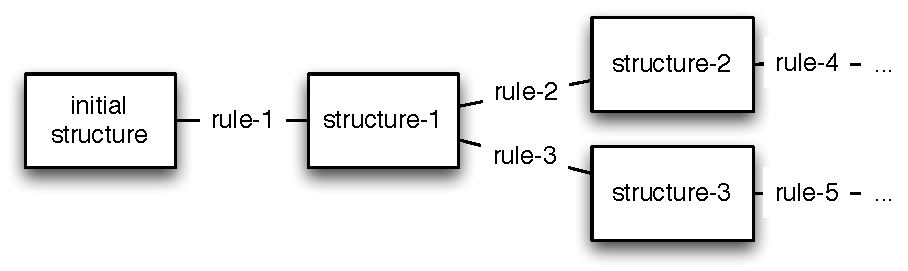
\includegraphics[width=.75\textwidth]{./frameworks/figures/fcg-search.pdf}
    \caption[Application of a rule-set]{Typical language processing in
      FCG is organised as a search process. A linguistic structure is
      being built up by applying a series of rules to it. When two
      (conflicting) rules could apply to the same structure, this
      leads to a split in the application tree.}
    \label{f:fcg-search}
  \end{center}
\end{figure}

\subsection{Coupled feature structures}
\label{s:coupled-feature-structures}
\is{coupled feature structure}

The linguistic structure that is being built up is represented as
\textsc{coupled feature structures}. Each coupled feature structure
consists of two feature structures or \textsc{poles}: one is defined in
the semantic domain and the other in the syntactic domain. Each
feature structure consists of a list of units, which are typically
reflected in both poles. Each unit consists of a list of feature-value
pairs which represent linguistic information. Special features,
\emph{sem-subunits} in the semantic pole and \emph{syn-subunits},
allow to specify hierarchical relations between units to construct
treelike relations between units.

FCG is open-ended to the features it can handle, but the features that
are typically used are: \emph{meaning}, \emph{referent}, and
\emph{sem-cat} in the semantic pole and \emph{form} and \emph{syn-cat}
in the syntactic pole. The \emph{meaning} feature refers to the
conceptual meaning of a certain unit, which can be expressed in any
formalism, including predicate logic or a semantic network in IRL. The
\emph{referent} is typically represented as a unique variable which is
bound to the (physical) entity that a unit (including all its
subunits) refers to. The \emph{form} feature contains all posible form
constraints, such as particular strings or word-order constraints
between its subunits. The \emph{syn-} and \emph{sem-cat} are
categories, either in the semantic or syntactic domain, that allow
other rules to specify which units to select for.

An example of a simplified linguistic structure for an utterance like
\textit{le ballon} is shown in Figure \ref{f:cfs-le-ballon} and its
bracketed notation is shown below. The semantic pole is shown on the
left and the syntactic pole on the right to show the structural
similarity between both poles.

\footnotesize
\ltitle{Example linguistic structure for "le ballon"}
\begin{lstlisting}
((top-unit                          ((top-unit
  (sem-subunits (det-np-unit)))       (syn-subunits (det-np-unit))
 (det-np-unit                        (det-np-unit
  (sem-subunits                       (syn-subunits 
   (ballon-unit le-unit))              (ballon-unit le-unit))
  (referent x)                        (form ((meets le-unit ballon-unit)))
  (meaning ((grounded x)))            (syn-cat 
  (sem-cat (object)))                  (determined-nounphrase)))
 (le-unit                            (le-unit 
  (referent x)                        (form 
  (meaning ((unique x)))               ((string le-unit "le")))
  (sem-cat (selector)))               (syn-cat (determiner)))
 (ballon-unit                        (ballon-unit 
  (referent x)                        (form 
  (meaning ((ball x)))                 ((string ballon-unit "ballon")))           
  (sem-cat (prototype))))             (syn-cat (noun))))
\end{lstlisting}
\normalsize

\begin{figure}[htbp]
  \begin{center}
    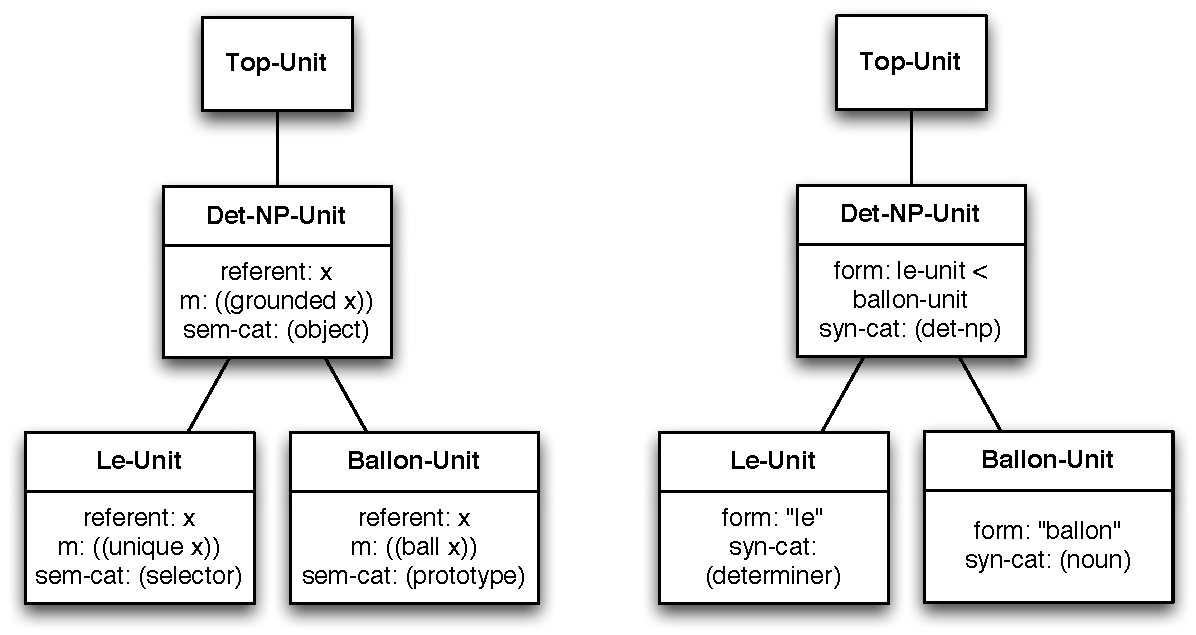
\includegraphics[width=.8\textwidth]{./frameworks/figures/cfs-le-ballon.pdf}
    \caption[Example coupled feature structure for \textit{le ballon}]{A
      graphical representation of the linguistic structure for \textit{le
      ballon}. The semantic pole is shown on the left, the syntactic
      pole on the right. Both poles are structurally very similar, but
      only contain features that are relevant in their domain.}
    \label{f:cfs-le-ballon}
  \end{center}
\end{figure}

\subsection{Application of a construction}

Now that we know how a linguistic structure is represented in FCG, we
can turn to the application of a construction to build up such a
structure. Like a linguistic structure, a construction is also
represented as a coupled-feature structure. The semantic pole of a
construction specifies how meaning has to be built up in parsing or
decomposed in production, and the syntactic pole how the form has to
be analysed in parsing or built in production. A construction also
typically contains more variables as it should be applicable to a wide
range of instantiated linguistic structures.

A construction is applied in three steps: a \textsc{matching phase}, a
\textsc{first merging phase} and a \textsc{second merging phase}. In
general, the matching phase checks whether the rule is applicable and
the two merging phases add new information to the linguistic structure
that is being built up. Although the matching phase is the most strict
one, all other phases can block the application of a rule if
conflicting information would already be present in the current
structure. More details on how matching and merging is exactly
implemented can be found in a background article
\citep{steels06unify}.

In production, it is the syntactic pole that is matched to the
syntactic pole of the current structure; in interpretation it is the
semantic pole that is matched to the current semantic pole. When the
matching phase has been successful, both poles of the rule are merged
into the current structure. The application of a rule is illustrated
in Figure \ref{f:fcg-rule-application}.

\begin{figure}[htb]
  \begin{center}
    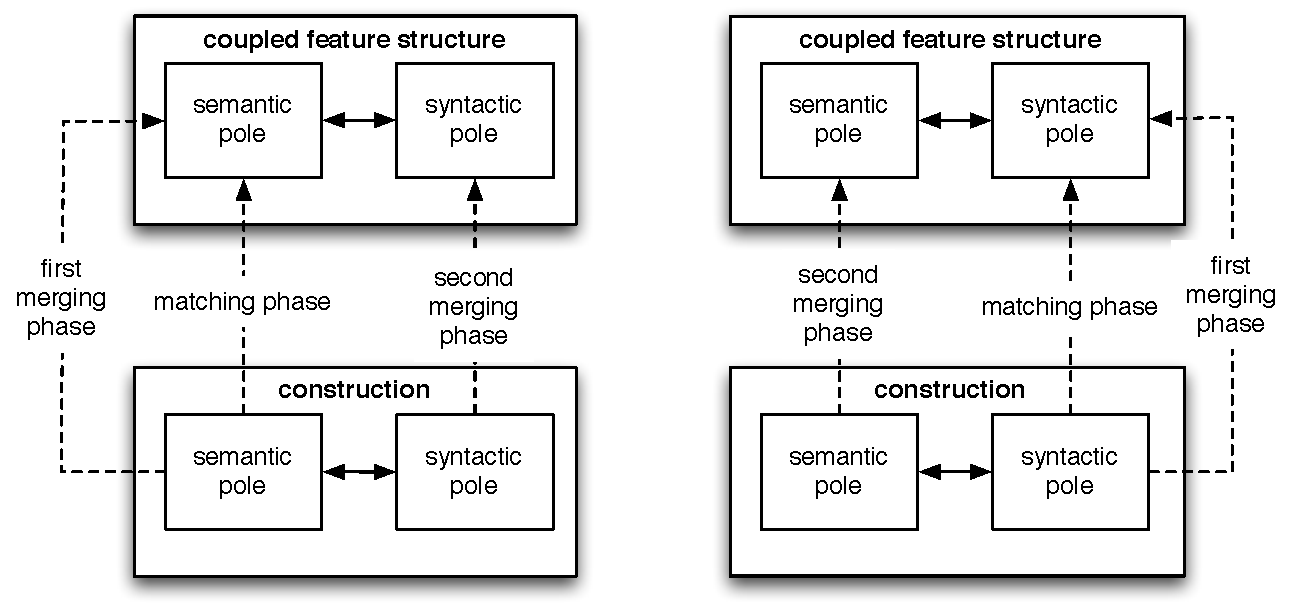
\includegraphics[width=\textwidth]{./frameworks/figures/fcg-rule-application.pdf}
    \caption[Application of a rule]{Rule application in FCG. Applying
      a rule consists of three phases: a matching phase and two
      merging phases. In production (left), the semantic pole is
      matched to check whether a rule is applicable. In interpretation
      (right), it is the syntactic pole that is matched. When the
      matching phase has been successful, both poles are merged into
      the coupled feature structure.}
    \label{f:fcg-rule-application}
  \end{center}
\end{figure}

\subsection{Structure building}
\is{FCG!structure building}
\is{structure building|see{FCG}}

The merging phases during the application of a construction can be
used to add new features to a unit or to add new values to a
particular feature of a particular unit, but more powerful structure
building operations are also possible. These operations can be used to
add new units to the structure, to change the hierarchy relations
between units and to move feature-value pairs from one unit to
another. All these operations are achieved through two operators: the
J-operator \citep{debeule05hierarchy} and the TAG-operator. The syntax
of these operators is shown below.


\footnotesize
\ltitle{Syntax of the TAG-Operator}
\begin{lstlisting}
(?unit
  (TAG ?tag-variable (feature-name feature-value)))
\end{lstlisting}

\ltitle{Syntax of the J-operator}
\begin{lstlisting}
((J ?focus-unit ?parent-unit (?child-unit-1 ... ?child-unit-n))
 ?tag-variable-1 
 ...
 ?tag-variable-n
 (feature-name-1 feature-value-1)
 ...
 (feature-name-n feature-value-n))
\end{lstlisting}
\normalsize

Units that are marked by the J-operator, or \textsc{J-units} for short,
are ignored in the matching phase, but receive special treatment
during the merging phase. The TAG-operator allows a construction to
bind a certain variable, \emph{?tag-variable}, to a certain
feature-value pair. Whenever this variable appears inside a J-unit of
the same rule, the bound feature-value pair will be moved to this
J-unit. The special treatment of a J-unit in the merging phase is as
follows:

\begin{enumerate}
\item if \emph{?focus-unit} is bound to a unit-name in the current
  structure, it will consider this unit to be in focus; if this
  variable is unbound, a new unit is created that will be in focus of
  this J-unit
\item the focus-unit will become a subunit of \emph{?parent-unit} and
  the optional \emph{?child-units} will become children of the
  focus-unit
\item the listed feature-value pairs will be merged into to the
  focus-unit
\item the feature-value pairs that are bound to the
  \emph{?tag-variables} will be moved from their original unit to the
  focus-unit
\end{enumerate}

\subsection{Linking through variable equalities}
\is{linking|see{FCG}}
\is{FCG!linking}

Once relations between several entities can be expressed in language,
hearers face an additional problem in figuring out what these
relations are. This is typically considered to be conveyed through
grammar. For example in a sentence like \textit{Jack hits Jill} English
grammar clearly conveys it is Jack who is the agent and Jill the
unfortunate recipient of the event, unlike the sentence \textit{Jill hits
Jack} in which the roles are reversed. Another example would be \textit{the
big block and the red ball} in which the hearer would need to figure
out it is the block which is big and the ball which is red. This
problem has been identified as the linking problem
\citep{steels05linking}.

In FCG this problem has been solved by first assuming that variables
introduced by different rules are different, but can be made equal
during the application of other grammatical rules. Let us consider the
phrase \textit{red ball} and assume the meaning is represented in predicate
logic. In parsing, the lexical constructions would introduce two
predicates, ``red(?x)'' and ``ball(?y)'', each introducing a different
variable. Another grammatical construction, which specifies that all
predicates referred to by adjectives and nouns that are part of the
same noun phrase should share the same variable, will make these
variables equal. The application of this rule transforms the
interpreted meaning in ``red(?x)'' and ``ball(?x)'' and hence solves the
linking problem for this small example.

\subsection{Application of an example construction}

I will now show the application of an example
NounAdjective-construction in interpretation. It illustrates both the
structure building operators and the linking problem. It will search
for two units, one of syntactical category \emph{noun} and the other
of syntactical category \emph{adjective} that occur next to each other
in the utterance parsed so far. When it has found two such units, it
introduces an intermediary unit and makes the variables of the
predicates in these two units equal through the referents of their
units. The coupled feature structure before and after application of
the construction is shown in Figure \ref{f:nounadj-application}.

\begin{figure}
  \begin{center}
    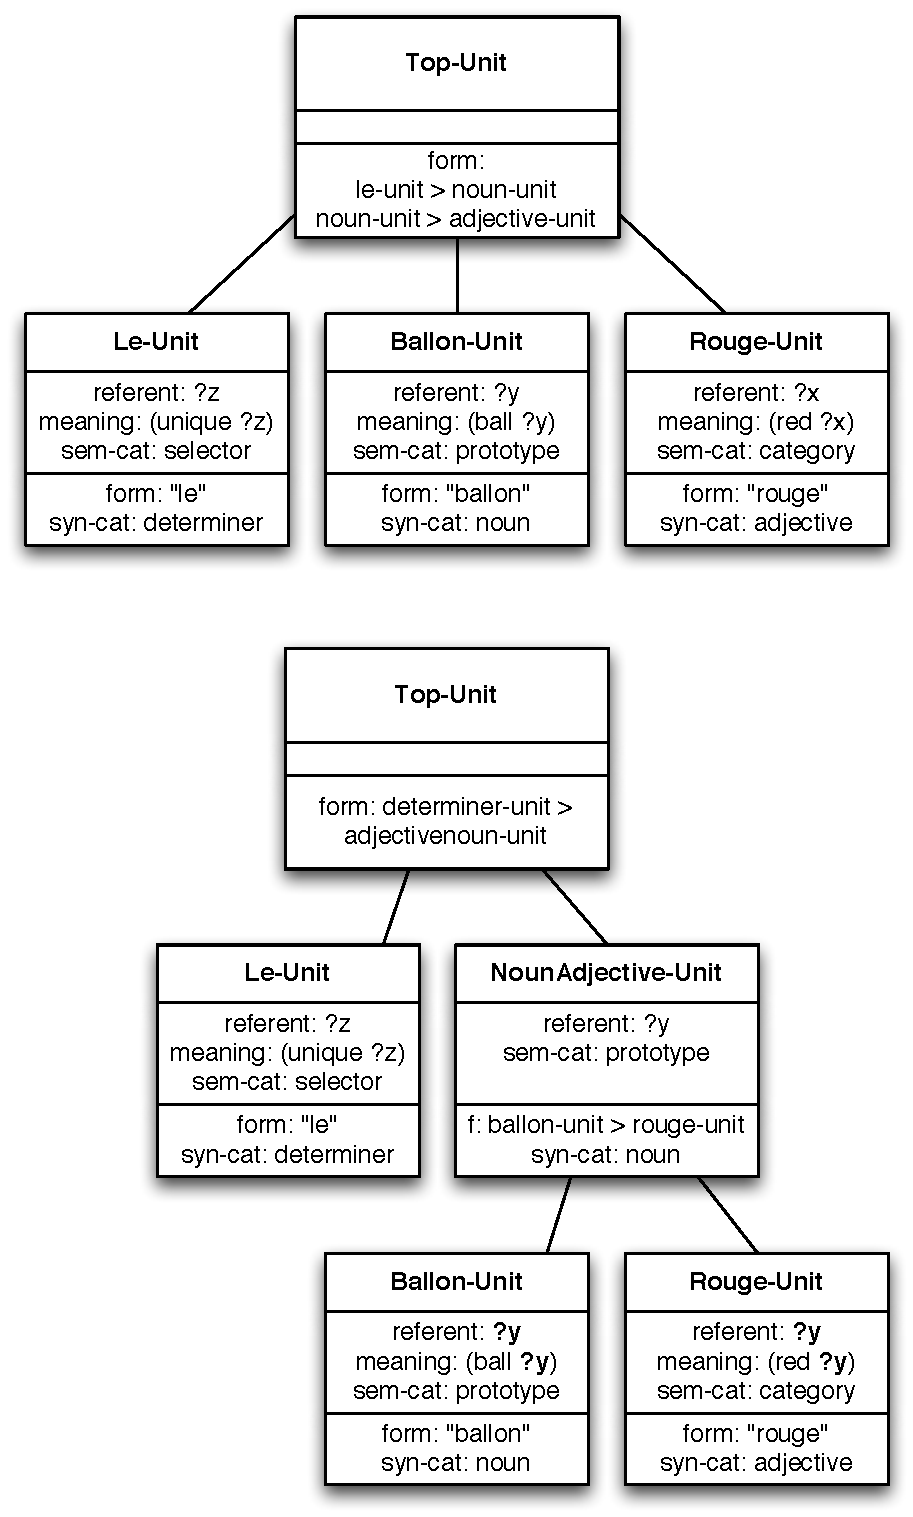
\includegraphics[width=.75\textwidth]{./frameworks/figures/nounadj-application.pdf}
    \caption[Coupled feature structures before and after the
    application of an example construction]{Coupled feature structures
      before (top) and after (bottom) the application of the
      NounAdjective construction in interpretation. It introduces a
      new unit which combines a Noun and an Adjective unit and makes
      the variables of their predicates equal through their
      referents. The coupled feature structures are now mapped on one
      structure which both contains semantic and syntactic
      information.}
    \label{f:nounadj-application}
  \end{center}
\end{figure}

I'll now step through the rule application of the rule in more
detail. In interpretation the utterance is de-rendered into a set of
form constraints: a set of strings, one for each word, and a set of
meets constraints between each consecutive pair of words. An example
for \textit{le ballon rouge} is given in the initial structure below. Note
that the semantic pole and syntactic pole are now shown under each
other and separated by a double arrow.

\footnotesize
\ltitle{Initial Structure}
\begin{lstlisting}
((top-unit))
<-->
((top-unit
 (form
   ((string le-unit "le")
    (string ballon-unit "ballon")
    (string rouge-unit "rouge")
    (meets le-unit ballon-unit)
    (meets ballon-unit rouge-unit)))))
\end{lstlisting}
\normalsize

Next the lexical constructions apply, which introduce for each string
a different unit (using the J-operator), which on the semantic side
introduces the corresponding meaning predicate together with their
referent and semantical category and on the syntactic side introduces
the appropriate syntactical categories. The coupled feature structure
after application of lexical constructions is shown below in bracketed
notation and in Figure \ref{f:nounadj-application} (top).

\footnotesize
\ltitle{Structure before application of the Noun-Adjective construction}
\begin{lstlisting}
((top-unit
  (sem-subunits (rouge-unit le-unit ballon-unit)))
 (rouge-unit
  (meaning ((red ?x)))
  (referent ?x)
  (sem-cat ((pom category))))
 (ballon-unit
  (meaning ((ball ?y)))
  (referent ?y)
  (sem-cat ((pom prototype))))
 (le-unit
  (meaning ((unique ?z)))
  (referent ?z)
  (sem-cat ((pom selector)))))
<-->
((top-unit
  (syn-subunits (rouge-unit le-unit ballon-unit))
  (form
   ((meets ballon-unit rouge-unit) 
    (meets le-unit ballon-unit))))
 (rouge-unit
  (form ((string rouge-unit "rouge")))
  (syn-cat ((pos adjective))))
 (le-unit 
  (form ((string le-unit "le"))) 
  (syn-cat ((pos determiner))))
 (ballon-unit
  (form ((string ballon-unit "ballon")))
  (syn-cat ((pos noun)))))
\end{lstlisting}
\normalsize

We are now ready to apply the Noun-Adjective construction which is
shown below. The first phase is the matching phase and as we are in
interpretation, this means the syntactic pole of the construction will
be matched against the syntactic pole of the current coupled feature
structure, which succeeds. There is only one adjective-unit and one
noun-unit, so this results one set of possible bindings:
\emph{((?parent-unit . top-unit) (?noun-unit . ballon-unit)
  (?adjective-unit . rouge-unit))}.

Matching succeeded, so we can now continue in the first merge phase,
in which the syntactic pole of the construction is merged into the
current feature structure. The syntactic pole contains only one J-unit
which will now be applied. As there is no binding for
\emph{?adj-noun-unit} yet, it will create a new unit that will be a
child of \emph{?parent-unit} (which in this application will be
\emph{top-unit} as can be seen in the bindings of the unification
phase) and which will have two children: \emph{ballon-unit} and
\emph{rouge-unit}. The feature-value pairs specified in the J-unit,
namely the syntactical category noun, will be added to this
unit. Finally the tag-variable \emph{?form} will be handled, which
moves the meets constraint between the \emph{ballon-unit} and the
\emph{rouge-unit} from \emph{top-unit} to the newly created unit.

\footnotesize
\ltitle{The Noun-Adjective construction}
\begin{lstlisting}
((?parent-unit
  (sem-subunits (== ?noun-unit ?adjective-unit)))
 (?noun-unit 
  (referent ?x) 
  (sem-cat (==1 (pom prototype))))
 (?adjective-unit
  (referent ?x)
  (sem-cat (==1 (pom category))))
 ((J ?adj-noun-unit ?parent-unit (?noun-unit ?adjective-unit))
  (referent ?x)
  (sem-cat (==1 (pom prototype)))))
<-->
((?parent-unit
  (syn-subunits (== ?noun-unit ?adjective-unit))
  (tag
   ?form
   (form (== (meets ?noun-unit ?adjective-unit)))))
 (?noun-unit 
  (syn-cat (==1 (pos noun))))
 (?adjective-unit 
  (syn-cat (==1 (pos adjective))))
 ((J ?adj-noun-unit ?parent-unit (?noun-unit ?adjective-unit))
  ?form
  (syn-cat (==1 (pos noun)))))
\end{lstlisting}
\normalsize

In the final merging phase, the semantic pole of the construction is
merged into the semantic pole of the current feature structure. Next
to creating a new unit similar to the unit created in the syntactic
pole, it ensures the variables of the predicates for ball and red will
be made equal. In the current structure they are available as the
referent of the \emph{ballon-unit} and the \emph{rouge-unit}, which
are equal in the \emph{?adjective-unit} and the \emph{?noun-unit} of
the Noun-Adjective construction. The merging phase will ensure that
these variables are equalised in the resulting feature structure,
which is shown below and in Figure \ref{f:nounadj-application}
(bottom).

\footnotesize
\ltitle{Structure after application in interpretation}
\begin{lstlisting}
((top-unit
  (sem-subunits (noun-adj-unit le-unit)))
 (noun-adj-unit
  (sem-subunits (rouge-unit ballon-unit))
  (referent ?y)
  (sem-cat ((pom prototype))))
 (le-unit
  (meaning ((unique ?z)))
  (referent ?z)
  (sem-cat ((pom selector))))
 (ballon-unit
  (meaning ((ball ?y)))
  (sem-cat ((pom prototype)))
  (referent ?y))
 (rouge-unit
  (meaning ((red ?y)))
  (sem-cat ((pom category)))
  (referent ?y)))
<-->
((top-unit 
  (syn-subunits (noun-adj-unit le-unit))
  (form ((meets le-unit noun-adj-unit))))
 (noun-adj-unit
  (form ((meets ballon-unit rouge-unit)))
  (syn-subunits (rouge-unit ballon-unit))
  (syn-cat ((pos noun))))
 (rouge-unit
  (form ((string rouge-unit "rouge")))
  (syn-cat ((pos adjective))))
 (le-unit 
  (form ((string le-unit "le"))) 
  (syn-cat ((pos determiner))))
 (ballon-unit
  (form ((string ballon-unit "ballon")))
  (syn-cat ((pos noun)))))
\end{lstlisting}
\normalsize
